% Rules for the HuroCup Obstacle Run Competition
% Jacky Baltes <jacky@cs.umanitoba.ca> 

\documentclass[12pt]{hurocup}

\begin{document}

\title{\HuroCup: Obstacle Run\\
  Laws of the Game 2008}


\author{Jacky Baltes\\
Autonomous Agents Laboratory\\
University of Manitoba\\
Winnipeg, Manitoba\\
Canada, R3T 2N2\\
Email: jacky@cs.umanitoba.ca\\
WWW: http://www.cs.umanitoba.ca/\~{ }jacky\\[5mm]
Kuo-Yang Tu\\
National Kaohsiung First University of Science and Technology\\
Kaohsiung City, R. O. C.\\
Email: tuky@ccms.nkfust.edu.tw\\
}

\maketitle

\begin{center}
 \includegraphics[width=0.7\linewidth]{Figures/obstacle-run-life}
\end{center}

\begin{abstract}
The following rules and regulations govern the Obstacle Run event in
\HuroCup, a robotic game and robotics benchmark problem for humanoid
robots.
%
\end{abstract}

\section*{Latest Version of the Rules for \HuroCup}
\label{sec:updates}

The latest official version of the rules of the game for \HuroCup\ is
always available from the FIRA \HuroCup\ website (http://www.fira.net).

\newpage

\section{Obstacle Run}
\label{subsec:obstacle-run} 

In the obstacle run challenge, the robot must move from one end of the
playing field to the other as quickly as possible.

There are three types of obstacles in the environment: (a) hole
obstacles that simulate holes in the floor, (b) wall obstacles which
can not be overcome, and (c) gate obstacles that a sufficiently mobile
robot can overcome by crawling under them.

\section{Changes in the Laws of \HuroCup\ Obstacle Run for 2008}

There are no significant changes between the 2008 and 2007 laws of the
obstacle run event.

\section{Laws of the Game: Obstacle Run}
\label{sec:laws-obstacle-run}

The following laws describe the specifics of the obstacle run
event. For general specifications relevant to all \HuroCup\ events
(e.g., robot dimensions, playing field and lighting, responsibility of
the referees) please refer to the general \HuroCup\ laws.

\law[OR]{The Field of Play}
\label{law:or-field}

\begin{lawlist}[OR]
\item The dimensions of the playing field are at least 430cm by
  200cm. 
\item There is a finish line marked on one side of the playing field.
  This side of the playing field is called the finish side. The
  opposite side of the playing field is called the start side. The two
  other sides are called side lines. The field of play is shown in
  Fig.~\ref{fig:obstacle-run}.  

  \begin{figure}
    \begin{center}
      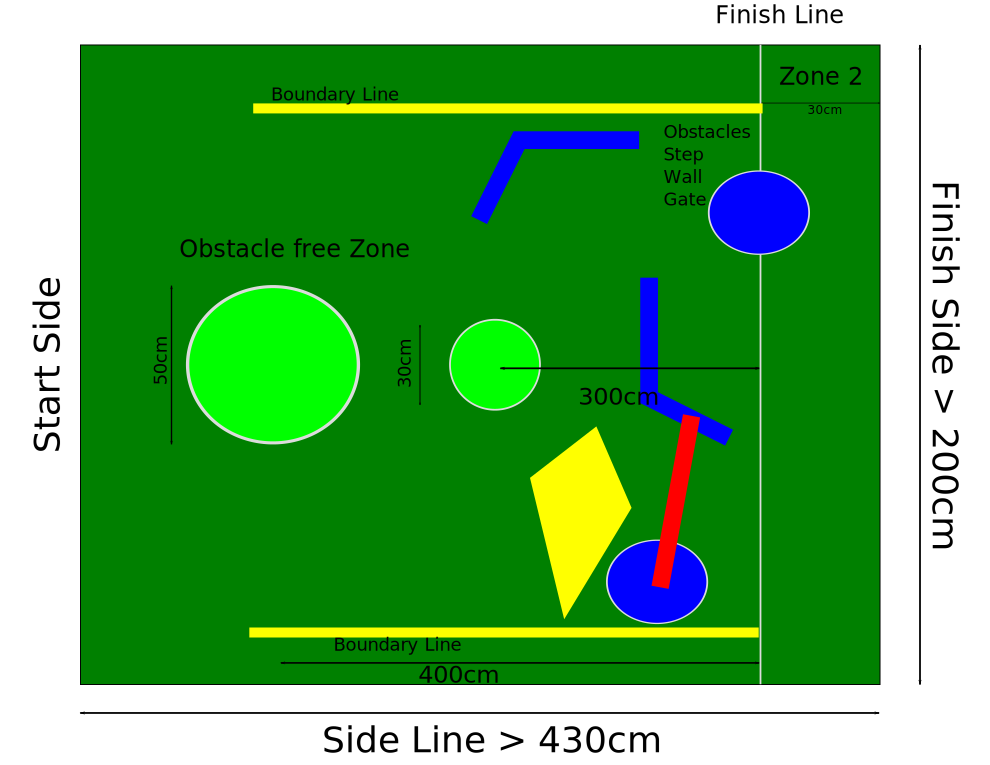
\includegraphics[width=0.7\textwidth]{Figures/obstacle-run}
    \end{center}
    \caption{The field of play for the obstacle run challenge}
    \label{fig:obstacle-run}
  \end{figure}

\item There is a 30cm zone behind the finish line, which is called the
  end zone.
\item \label{or-start-points} There are two start points marked on
  the playing field. The start points are approximately in the center
  of the playing field. The distance between the start point and the
  finish line depends on the category of the robot.
  \begin{enumerate}
  \item The start point for small robots is 300 cm in front of the
    finish line. 
  \item The start point for large robots is 400 cm in front of the
    finish line. 
  \end{enumerate}
\item Teams may place small coloured markers in the area behind the
  end zone to guide the robot as long as they do not interfere with
  other teams.
\end{lawlist}

\law[OR]{Obstacles}
\label{or-obstacles}

\begin{lawlist}[OR]

\item \label{or-obs-hole} A hole obstacle is a thin obstacle on the
  playing field. The shape and size of the hole obstacles is
  undefined. The colour of a hole obstacle is yellow.

\item \label{or-obs-wall} A wall obstacle is an obstacle that is
placed on the floor and has a height of approximately 30cm. It has
a minimum length of 40cm. The colour of a wall obstacle is blue.

\item \label{or-obs-gate} A gate obstacle is an obstacle that is
placed at a height of approximately 30cm. It has
a minimum length of 40cm. The colour of a gate obstacle is red.

\item The following figure shows pictures of suitable obstacle.

  \begin{figure}
    \begin{center}
      \begin{tabular}{cc}
        \includegraphics[width=0.4\textwidth]{Figures/wall-obstacles} &
        \includegraphics[width=0.4\textwidth]{Figures/gate-obstacle} \\
      \end{tabular}
      \caption{Wall and gate obstacles used in the obstacle run}
      \label{fig:obstacles}
    \end{center}
  \end{figure}

\item The referee or a person designated by the referee shall place
  at least five obstacles (see~\ref{or-obstacles}) at random in the
  playing field.

\item \label{obs-place1} The obstacles may be placed anywhere on the
  playing field from the start point to the finish line given the
  following constraints:

  \begin{itemize} 
  \item a circular region with a radius of at least 30cm and 50cm
    for small and large robots respectively around the starting
    point is free of obstacles,
  \item at least one of the obstacles shall be in the direct path of the
    robot to the finish line,
  \item there is at least one free walkable path from the start point to the
    finish line. That is, a circle with a diameter of 40cm can be moved
    from the start point to the finish line without touching any
    obstacle or passing underneath or over any of the obstacles. Note
    that this does not imply that the minimum distance between two
    obstacles is at least 40cm. Some obstacles may be closer together than
    40cm as can be seen in Fig.~\ref{fig:obstacle-run}. 
  \end{itemize}
\end{lawlist}

\begin{decisions}

\item A hole obstacle is supposed to simulate holes in the playing
  field. Therefore, a robot is not allowed to touch such an
  obstacle. However, the robot is allowed to step over a thin hole
  obstacle

\end{decisions}

\law[OR]{Number of Robots}

\begin{lawlist}[OR]
\item A single robot competes in a match.
\end{lawlist}

\law[OR]{The Players}

Please refer to the general \HuroCup\ laws for a description of
the players.

\law[OR]{The Referee}

Please refer to the general \HuroCup\ laws for a description of
the referee.

\law[OR]{The Assistant Referee}

Please refer to the general \HuroCup\ laws for a description of
the assitant referee.

\law[OR]{Game Play}

\begin{lawlist}[OR]

\item A single robot is designated the runner. All other robots
  must be outside of the playing field.
\item The only robot allowed to move during a run is the
  designated runner.
\item Each robot may have at most one human handler associated with
  it. 
\item \label{or-handler5} The human handlers are not allowed to
  interfere in any way with other robots, the referee, or other human
  handlers.
\item \label{or-handler6} A human handler may only enter the playing
  field or touch his/her robot with the permission of the referee.
\item At the beginning of the competition, the designated runner must
  be at the start point for its respective category. The runner must
  face forward. (See~\ref{or-start-points}).
\item After the robot has been placed, the obstacles will be
  distributed by the referee according
  to~\ref{obs-place1}.
\item The referee will signal the start of the competition by blowing
  the whistle.
\item A robot is not allowed to leave the playing field as defined
  in~\ref{law:or-field}. 
\item A robot has crossed the finish line when either foot of the
  robot crosses the finish plane and touches the ground in the end
  zone. The finish plane is the plane which intersects the playing
  field at a 90 degree angle at the back of the finish line.
\item The handler shall remove his/her assigned robot as soon as
  possible from the end zone after it has crossed the finish line.
\item The end of the competition is signaled by the referee by
  blowing the whistle a second time.
  The referee terminates the competition if
  \begin{itemize}
  \item the robot has crossed the finish line,
  \item the maximum duration of the competition (three minutes) has
    elapsed. 
  \item the robot is immobilized by a technical defect,
  \item the robot leaves the playing field,
  \item the robot touches one of the wall, hole, or gate obstacles (In
    case the obstacle was moved by the robot, the obstacle will be
    repositioned by the referee),
  \item at least two minutes have elapsed since the start of the
    competition and it is unlikely in the opinion of the referee that
    the robot will cross the finish line within the minute,
  \end{itemize}
\end{lawlist}

\law[OR]{Method of Scoring}

\begin{lawlist}[OR]
\item At the end of the run, another robot will be designated the
  runner.
\item There are five rounds in the competition. Each round consists of
  all robots being designated the runner exactly once. Each robot
  receives one point for each run in which it manages to cross the
  finish line.
\item Any robot that has not reached the finish line at least once is automatically
  awarded 0 rank.
\item Among the robots that have reached the finish line at least
  once, the robots are ranked (i.e., 1st place, 2nd place) based on
  the greater number of successful runs.

\item The point allocation for robots is as follows:
  \begin{itemize}
  \item The first ranked robot is awarded $10$ points.
  \item The second ranked robot is awarded $8$ points.
  \item The third ranked robot is awarded $6$ points.
  \item The fourth, fifth, sixth, and seventh place robots are awarded
    $4$,$3$,$2$, and $1$ point respectively.  A summary of the point
    allocation for placings is shown in table~\ref{point-allocation}.

    \begin{table}
      \begin{center}
        \begin{tabular}{l|l}
          \hline
          Place & Points scored \\
          \hline
          1 (Winner) & 10 \\
          2          & 8 \\
          3          & 6 \\
          4          & 4 \\
          5          & 3 \\
          6          & 2 \\
          7          & 1 \\
          8, 9, ...  & 0 \\
          \hline
        \end{tabular}
      \end{center}
      \caption{Point allocation for placings in the \HuroCup\ events.}
      \label{point-allocation}
    \end{table}
  \end{itemize}

\item In case of a tie between $n$ robots with rank $k$, all robots
 will be awarded rank $k$ and receive the average of the scores for
 ranks $k$ to $k+n$.  For example, if the robots $A,B,C,D$ scored $10,
 8, 8, 4$ goals respectively, then robot $A$ will be declared the
 winner (1st place) and receive 10 points, both robots $B$ and $C$
 will be declared 2nd place finishers and receive $(8+6)/2=7$, and
 robot $D$ will be declared the fourth place finisher and receive $4$
 points.

\end{lawlist}
\end{document}


% *** Local Variables: ***
% *** mode: LaTeX ***
% *** mode: outline-minor ***
% *** mode: auto-fill ***
% *** outline-regexp: "% !\\|\\\\\\(sub\\)*section" ***
% *** TeX-command-default: "LaTeX PDF" ***
% *** End: ***
